
\documentclass{article}

\author{GT RoboJackets}
\title{RoboCup SSL Motion Control}


\usepackage{graphicx}
\usepackage{hyperref}

\begin{document}

\maketitle



\begin{figure}[p]
	\centering
	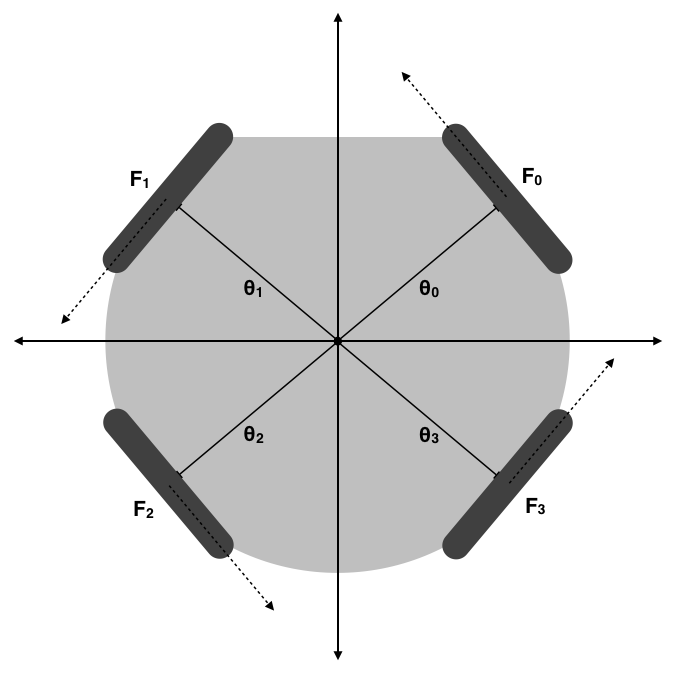
\includegraphics[width=4in]{WheelDiagram.png}
	\caption{Wheel Diagram}
	\label{fig:wheel_diagram}
\end{figure}


\section*{Intro}

The goal of 'motion control' is that given a particular path, we command the robots such that they follow it as accurately as possible.  We want our robots to move quickly and have very little error and overshoot.

A path is a function of the robot's position ($x$,$y$,$\theta$) given time.  It could be a line, a circle, a bezier curve, or any other shape as long as it doesn't exceed the physical constraints of the robot.  A path should never require the robot to move or accelerate faster than it is physically capable of.  Creating these paths is a tough problem in itself, but will not be considered here - that is a problem that we will handle separately, although it's definitely related to motion control.  The motion control module assumes that the given path is valid and doesn't exceed the constraints of the robot.


\section*{Sensors}

We measure the robot's movement using a few different sensors.

\subsection*{Cameras}
There are two to four cameras above the field that, after having their raw images processed by ssl-vision, give us the positions and angles of all robots on the field at a frequency of about 60Hz.

\subsection*{Wheel Encoders}
Our 2008 and 2011 model robots have hall-effect sensors that serve as very low resolution encoders to tell us how much each wheel has rotated.
The new 2015 fleet of robots will have high-resolution encoders on each wheel.
By measuring the change in position of each wheel over time, we can calculate the velocity.

\subsection*{MPU}
Each robot has an on-board Motion Processing Unit (MPU) that tells us the acceleration and angular velocity of the robot.  This can be integrated over time to give us the change in position and angle.


\subsection*{Control Loop}
The 'soccer' program on the field laptop accepts vision data from ssl-vision to get the position of each robot.  We then reconcile that with the target path that each robot should be following and send out velocity commands to each robot wirelessly.  The robots then use their on-board sensors to execute the velocity commands as well as possible.  By continually sending new commands to the robots, we can get them to follow arbitrary paths.

\subsubsection*{Delay}
There is delay between the cameras and the 'soccer' program as well as between 'soccer' and the robots receiving commands.  How do we handle it?


\section*{Forces}

Find the total force and torque on the robot.  Assume $R$ is the distance from the center of the robot to the center of one of the wheels and that they are all the same distance from the center. See figure \ref{fig:wheel_diagram}.

$\Sigma_F = F_0 + F_1 + F_2 + F_3 + F_4$

$\tau = R*(F_0+F_1+F_2+F_3)$

From this we can find the accelerations of the robot:

$a = \frac{1}{M} (F_0 + F_1 + F_2 + F_3)$

$\dot{\omega} = \frac{R}{I}(f_0 + f_1 + f_2 + f_3)$

Where $M $ is the mass of the robot and $I$ is the rotational inertia and the lowercase 'f's are the magnitudes of the forces.


Next, we put these together in matrix form using what is called the "force-coupling matrix".  Note: this was borrowed from \url{http://people.idsia.ch/~foerster/2006/1/omnidrive_kiart_preprint.pdf}.

\begin{math}
\left( \begin{array}{c}
	a_x \\
	a_y \\
	\dot{\omega}
\end{array} \right)
= \frac{1}{M}
\left( \begin{array}{cccc}
	-\sin(\theta_0) & -\sin(\theta_1) & -\sin(\theta_2) & -\sin(\theta_3) \\
	\cos(\theta_0) & \cos(\theta_1) & \cos(\theta_2) & \cos(\theta_3) \\
	\frac{M R}{I} & \frac{M R}{I} & \frac{M R}{I} & \frac{M R}{I} \\
\end{array} \right)
\left( \begin{array}{c}
	f_0 \\
	f_1 \\
	f_2 \\
	f_3 \\
\end{array} \right)
\end{math}


\end{document}
